
\documentclass[12pt]{article}
\usepackage[a4paper, margin=2cm]{geometry} %Annina style
\usepackage[utf8]{inputenc}
\usepackage{graphicx}
% \usepackage[style=ieee]{biblatex}  % Set bibliography style to IEEE
% \usepackage[backend=biber,style=numeric]{biblatex}
\usepackage{amsmath}
\usepackage{amsfonts}
\usepackage{amssymb}
\usepackage{hyperref}
\usepackage{xurl}
\usepackage{setspace} % Add this package for spacing commands
\usepackage[numbers]{natbib} % Add this package for bibliography management
\usepackage{float}
\usepackage{listings}
\usepackage{xcolor}
\usepackage{caption} % Required for using \captionof
\usepackage{algorithm} 
\usepackage{algorithmicx} 
\usepackage{algpseudocode}
\usepackage{tikz}
\usetikzlibrary{arrows.meta}
\numberwithin{equation}{section}

\renewcommand{\lstlistingname}{Code}
\lstset{ 
    language=Python, 
    basicstyle=\ttfamily\small, 
    keywordstyle=\color{blue}, 
    stringstyle=\color{red}, 
    commentstyle=\color{green}, 
    showstringspaces=false,
    numbers=left,
    numberstyle=\tiny\color{gray},
    frame=single,
    breaklines=true
}
\setlength{\parindent}{0pt}

\title{XAI: Cluster Variational Inference Reports}
\author{Jack Li}
\date{February 23, 2025}

\begin{document}

\onehalfspacing  % Or \doublespacing

\maketitle

\section{Derivation of the ELBO for a Variational Autoencoder}

In a Variational Autoencoder (VAE), we aim to maximize the marginal log-likelihood of the observed data \( x \), denoted \( \log p(x) \), over a dataset. However, computing \( p(x) = \int p(x, z) \, dz = \int p(x | z) p(z) \, dz \) directly is intractable due to the integral over the latent variable \( z \). Variational inference introduces an approximate posterior \( q(z | x) \) to address this. The Evidence Lower Bound (ELBO) provides a tractable objective to optimize. Here, we derive it.

\subsection{Starting Point: Marginal Log-Likelihood}
Consider the marginal log-likelihood of the data:
\begin{equation}
\log p(x) = \log \int p(x, z) \, dz.
\label{eq:marginal_log_likelihood}
\end{equation}
Since this integral is intractable, we introduce a variational distribution \( q(z | x) \) over the latent variables \( z \), which approximates the true posterior \( p(z | x) \).

\subsection{Introducing \( q(z | x) \)}
Using the definition of expectation, we rewrite \( \log p(x) \) by incorporating \( q(z | x) \):
\begin{equation}
\log p(x) = \log \int p(x, z) \frac{q(z | x)}{q(z | x)} \, dz = \log \mathbb{E}_{q(z | x)} \left[ \frac{p(x, z)}{q(z | x)} \right].
\label{eq:expectation}
\end{equation}

\subsection{Applying Jensen's Inequality}
Since the logarithm is a concave function, Jensen's inequality states that \( \log \mathbb{E}[f(z)] \geq \mathbb{E}[\log f(z)] \) for any random variable \( z \) and function \( f(z) \). Applying this:
\[
\log p(x) = \log \mathbb{E}_{q(z | x)} \left[ \frac{p(x, z)}{q(z | x)} \right] \geq \mathbb{E}_{q(z | x)} \left[ \log \frac{p(x, z)}{q(z | x)} \right].
\]
This lower bound is the ELBO, denoted \( \mathcal{L}(x) \):
\begin{equation}
\mathcal{L}(x) = \mathbb{E}_{q(z | x)} \left[ \log \frac{p(x, z)}{q(z | x)} \right].
\label{eq:elbo}
\end{equation}
Equality holds when \( q(z | x) = p(z | x) \), but since \( p(z | x) \) is intractable, we optimize \( q(z | x) \) to make the bound as tight as possible.

\subsection{Expanding the ELBO}
Now, expand the joint distribution \( p(x, z) = p(x | z) p(z) \) inside the expectation:
\begin{equation}
\mathcal{L}(x) = \mathbb{E}_{q(z | x)} \left[ \log \frac{p(x | z) p(z)}{q(z | x)} \right].
\end{equation}
Using the linearity of expectation:
\begin{equation}
\mathcal{L}(x) = \mathbb{E}_{q(z | x)} \left[ \log p(x | z) + \log p(z) - \log q(z | x) \right].
\end{equation}
This splits into:
\begin{equation}
\mathcal{L}(x) = \mathbb{E}_{q(z | x)} \left[ \log p(x | z) \right] + \mathbb{E}_{q(z | x)} \left[ \log \frac{p(z)}{q(z | x)} \right].
\label{eq:elbo_split}
\end{equation}

\subsection{Rewriting with KL Divergence}
Recognize that the second term is the negative Kullback-Leibler (KL) divergence between \( q(z | x) \) and \( p(z) \):
\[
\mathbb{E}_{q(z | x)} \left[ \log \frac{p(z)}{q(z | x)} \right] = - \mathbb{E}_{q(z | x)} \left[ \log \frac{q(z | x)}{p(z)} \right] = - D_{\text{KL}}(q(z | x) \| p(z)).
\]
Thus, the ELBO becomes:
\begin{equation}
\mathcal{L}(x) = \mathbb{E}_{q(z | x)} \left[ \log p(x | z) \right] - D_{\text{KL}}(q(z | x) \| p(z)).
\label{eq:elbo_kl}
\end{equation}

\subsection{Interpretation}
- The first term, \( \mathbb{E}_{q(z | x)} \left[ \log p(x | z) \right] \), is the expected log-likelihood of the data under the generative model, often interpreted as a reconstruction term when \( p(x | z) \) is parameterized (e.g., as a Gaussian or Bernoulli distribution).
- The second term, \( - D_{\text{KL}}(q(z | x) \| p(z)) \), is a regularization term that encourages \( q(z | x) \) to be close to the prior \( p(z) \), typically a standard normal \( \mathcal{N}(0, I) \).

\subsection{Relation to \( \log p(x) \)}
To confirm, relate \( \mathcal{L}(x) \) back to \( \log p(x) \):
\begin{equation}
\log p(x) = \mathbb{E}_{q(z | x)} \left[ \log \frac{p(x, z)}{q(z | x)} \right] + D_{\text{KL}}(q(z | x) \| p(z | x)).
\end{equation}
Since \( D_{\text{KL}}(q(z | x) \| p(z | x)) \geq 0 \) (KL divergence is non-negative), we have:
\begin{equation}
\log p(x) = \mathcal{L}(x) + D_{\text{KL}}(q(z | x) \| p(z | x)) \geq \mathcal{L}(x).
\label{eq:log_p_x}
\end{equation}
This shows \( \mathcal{L}(x) \) is indeed a lower bound on \( \log p(x) \), tightened by minimizing the KL divergence to the true posterior.

\subsection{Final ELBO Formula}
The ELBO, as used in VAEs, is:
\begin{equation}
\mathcal{L}(x) = \mathbb{E}_{q(z | x)} \left[ \log p(x | z) \right] - D_{\text{KL}}(q(z | x) \| p(z)).
\label{eq:final_elbo}
\end{equation}
In practice, \( q(z | x) \) is parameterized (e.g., as \( \mathcal{N}(\mu(x), \sigma^2(x)) \)) by an encoder network, and \( p(x | z) \) by a decoder network, with the KL term often computed analytically when \( p(z) = \mathcal{N}(0, I) \).

\section{Starting Point: The Final ELBO}

We begin with the Evidence Lower Bound (ELBO) for a Variational Autoencoder (VAE) where the latent variable is composed of \( z \) and \( c \), i.e., the joint latent representation is \( (z, c) \). The approximate posterior is factorized as \( q(z, c | x) = q(c | z) q(z | x) \), and the prior is factorized as \( p(z, c) = p(z | c) p(c) \). The ELBO is given by:

\begin{equation}
\mathcal{L}(x) = \mathbb{E}_{q(z, c | x)} \left[ \log p(x | z, c) \right] - D_{\text{KL}}(q(z, c | x) \| p(z, c))
\label{eq:elbo_zc}
\end{equation}

Our goal is to expand this expression using the specified factorizations.

\subsection{Step 1: Expand the Reconstruction Term}

The first term is the expected log-likelihood of the data \( x \) under the approximate posterior:

\[
\mathbb{E}_{q(z, c | x)} \left[ \log p(x | z, c) \right]
\]

Given \( q(z, c | x) = q(c | z) q(z | x) \), this expectation is over both \( z \) and \( c \), where \( z \sim q(z | x) \) and \( c \sim q(c | z) \). For continuous variables, this is a double integral:

\[
\mathbb{E}_{q(z, c | x)} \left[ \log p(x | z, c) \right] = \iint q(z | x) q(c | z) \log p(x | z, c) \, dz \, dc
\]

We compute this iteratively:
\begin{itemize}
    \item \textbf{Inner Integral}: For a fixed \( z \),
    \[
    \mathbb{E}_{q(c | z)} \left[ \log p(x | z, c) \right] = \int q(c | z) \log p(x | z, c) \, dc
    \]
    \item \textbf{Outer Integral}: Then over \( z \),
    \[
    \mathbb{E}_{q(z | x)} \left[ \mathbb{E}_{q(c | z)} \left[ \log p(x | z, c) \right] \right] = \int q(z | x) \left[ \int q(c | z) \log p(x | z, c) \, dc \right] \, dz
    \]
\end{itemize}

This nested form reflects the sampling process: first \( z \) from \( q(z | x) \), then \( c \) from \( q(c | z) \).

\subsection{Step 2: Expand the KL Divergence Term}

The second term is the KL divergence:

\[
D_{\text{KL}}(q(z, c | x) \| p(z, c)) = \iint q(z, c | x) \log \frac{q(z, c | x)}{p(z, c)} \, dz \, dc
\]

Substitute the factorizations:
- \( q(z, c | x) = q(c | z) q(z | x) \),
- \( p(z, c) = p(z | c) p(c) \).

Thus:

\[
D_{\text{KL}}(q(z, c | x) \| p(z, c)) = \iint q(c | z) q(z | x) \log \frac{q(c | z) q(z | x)}{p(z | c) p(c)} \, dz \, dc
\]

Split the logarithm:

\[
\log \frac{q(c | z) q(z | x)}{p(z | c) p(c)} = \log q(c | z) + \log q(z | x) - \log p(z | c) - \log p(c)
\]

So:

\[
D_{\text{KL}}(q(z, c | x) \| p(z, c)) = \iint q(c | z) q(z | x) \left[ \log q(c | z) + \log q(z | x) - \log p(z | c) - \log p(c) \right] \, dz \, dc
\]

Separate into four integrals:
\begin{enumerate}
    \item \(\iint q(c | z) q(z | x) \log q(c | z) \, dz \, dc = \mathbb{E}_{q(z | x)} \left[ \mathbb{E}_{q(c | z)} \left[ \log q(c | z) \right] \right]\),
    \item \(\iint q(c | z) q(z | x) \log q(z | x) \, dz \, dc = \mathbb{E}_{q(z | x)} \left[ \log q(z | x) \right]\) (since \(\int q(c | z) \, dc = 1\)),
    \item \(-\iint q(c | z) q(z | x) \log p(z | c) \, dz \, dc = -\mathbb{E}_{q(z | x)} \left[ \mathbb{E}_{q(c | z)} \left[ \log p(z | c) \right] \right]\),
    \item \(-\iint q(c | z) q(z | x) \log p(c) \, dz \, dc = -\mathbb{E}_{q(z | x)} \left[ \mathbb{E}_{q(c | z)} \left[ \log p(c) \right] \right]\).
\end{enumerate}

Group terms to form KL-like expressions:
- First and third: \(\mathbb{E}_{q(z | x)} \left[ D_{\text{KL}}(q(c | z) \| p(z | c)) \right]\) doesn’t directly apply due to mismatched conditionals, so we compute the full form later.

Instead, recompute directly:

\[
D_{\text{KL}} = \mathbb{E}_{q(z | x)} \left[ \mathbb{E}_{q(c | z)} \left[ \log \frac{q(z | x) q(c | z)}{p(z | c) p(c)} \right] \right]
\]

Factor:

\[
= \mathbb{E}_{q(z | x)} \left[ \log q(z | x) - \mathbb{E}_{q(c | z)} \left[ \log p(z | c) \right] + \mathbb{E}_{q(c | z)} \left[ \log \frac{q(c | z)}{p(c)} \right] \right]
\]

The last term is:

\[
\mathbb{E}_{q(c | z)} \left[ \log \frac{q(c | z)}{p(c)} \right] = D_{\text{KL}}(q(c | z) \| p(c))
\]

So:

\[
D_{\text{KL}}(q(z, c | x) \| p(z, c)) = \mathbb{E}_{q(z | x)} \left[ \log q(z | x) - \mathbb{E}_{q(c | z)} \left[ \log p(z | c) \right] + D_{\text{KL}}(q(c | z) \| p(c)) \right]
\]

\subsection{Step 3: Combine into the ELBO}

Substitute both terms into the ELBO:

\[
\mathcal{L}(x) = \mathbb{E}_{q(z | x)} \left[ \mathbb{E}_{q(c | z)} \left[ \log p(x | z, c) \right] \right] - \mathbb{E}_{q(z | x)} \left[ \log q(z | x) - \mathbb{E}_{q(c | z)} \left[ \log p(z | c) \right] + D_{\text{KL}}(q(c | z) \| p(c)) \right]
\]

Distribute the expectation:

\[
\mathcal{L}(x) = \mathbb{E}_{q(z | x)} \left[ \mathbb{E}_{q(c | z)} \left[ \log p(x | z, c) \right] - \log q(z | x) + \mathbb{E}_{q(c | z)} \left[ \log p(z | c) \right] - D_{\text{KL}}(q(c | z) \| p(c)) \right]
\]

\section{Explaining the Inequality}

In probabilistic modeling, such as variational autoencoders (VAEs), we often encounter expectations of KL divergences over latent variables. Here, we explain why the inequality

\[
\mathbb{E}_{q(z|x)} \left[ D_{\text{KL}}(q(c|z) || p(c)) \right] \geq D_{\text{KL}}(q(c|x) || p(c))
\]

holds, where:
\begin{itemize}
    \item \( x \) is the observed data,
    \item \( z \) and \( c \) are latent variables,
    \item \( q(z|x) \) is the approximate posterior distribution of \( z \) given \( x \),
    \item \( q(c|z) \) is the conditional distribution of \( c \) given \( z \),
    \item \( q(c|x) = \int q(c|z) q(z|x) \, dz \) is the marginal distribution of \( c \) given \( x \),
    \item \( p(c) \) is a prior distribution over \( c \), assumed to be independent of \( x \) and \( z \).
\end{itemize}

\subsection{Definition of KL Divergence}

The Kullback-Leibler (KL) divergence between two distributions \( p \) and \( q \) over a variable \( u \) is defined as:

\[
D_{\text{KL}}(p(u) || q(u)) = \int p(u) \log \frac{p(u)}{q(u)} \, du
\]

It measures the difference between \( p(u) \) and \( q(u) \) and is always non-negative (\( D_{\text{KL}} \geq 0 \)), with equality if and only if \( p(u) = q(u) \) almost everywhere.

\subsection{Left-Hand Side: Expected KL Divergence}

The left-hand side, \(\mathbb{E}_{q(z|x)} \left[ D_{\text{KL}}(q(c|z) || p(c)) \right]\), is the expectation of the KL divergence between \( q(c|z) \) and \( p(c) \) over \( z \) drawn from \( q(z|x) \):

\[
\mathbb{E}_{q(z|x)} \left[ D_{\text{KL}}(q(c|z) || p(c)) \right] = \int q(z|x) D_{\text{KL}}(q(c|z) || p(c)) \, dz
\]

Substitute the definition of KL divergence:

\[
D_{\text{KL}}(q(c|z) || p(c)) = \int q(c|z) \log \frac{q(c|z)}{p(c)} \, dc
\]

So:

\[
\mathbb{E}_{q(z|x)} \left[ D_{\text{KL}}(q(c|z) || p(c)) \right] = \int q(z|x) \left[ \int q(c|z) \log \frac{q(c|z)}{p(c)} \, dc \right] \, dz
\]

This represents the average divergence between \( q(c|z) \) and \( p(c) \), where \( q(c|z) \) varies with \( z \), and the expectation accounts for the distribution of \( z \) given \( x \).

\subsection{Right-Hand Side: Marginal KL Divergence}

The right-hand side, \( D_{\text{KL}}(q(c|x) || p(c)) \), is the KL divergence between the marginal distribution \( q(c|x) \) and \( p(c) \):

\[
D_{\text{KL}}(q(c|x) || p(c)) = \int q(c|x) \log \frac{q(c|x)}{p(c)} \, dc
\]

First, compute \( q(c|x) \) by marginalizing over \( z \):

\[
q(c|x) = \int q(c, z | x) \, dz = \int q(c|z) q(z|x) \, dz
\]

Thus:

\[
D_{\text{KL}}(q(c|x) || p(c)) = \int \left[ \int q(c|z) q(z|x) \, dz \right] \log \frac{\int q(c|z) q(z|x) \, dz}{p(c)} \, dc
\]

This measures the divergence between the averaged distribution \( q(c|x) \) and \( p(c) \).

\subsection{Applying Jensen's Inequality}

To show the inequality, recognize that the KL divergence \( D_{\text{KL}}(p || q) \) is a convex function with respect to \( p \). Consider the KL divergence as a functional of the distribution \( q(c|z) \). The left-hand side takes the expectation of this convex function over \( z \), while the right-hand side applies the KL divergence to the expected (or averaged) distribution \( q(c|x) \).

By Jensen's inequality, for a convex function \( f \) and a random variable \( Z \):

\[
\mathbb{E}[f(Z)] \geq f(\mathbb{E}[Z])
\]

Define \( f(q(c)) = D_{\text{KL}}(q(c) || p(c)) \), where \( q(c) \) is a distribution over \( c \). Here, \( q(c|z) \) is a distribution parameterized by \( z \), and \( z \sim q(z|x) \). The expectation of \( q(c|z) \) over \( z \) is:

\[
\mathbb{E}_{q(z|x)} [q(c|z)] = \int q(z|x) q(c|z) \, dz = q(c|x)
\]

Applying Jensen's inequality:

\[
\mathbb{E}_{q(z|x)} \left[ D_{\text{KL}}(q(c|z) || p(c)) \right] \geq D_{\text{KL}} \left( \mathbb{E}_{q(z|x)} [q(c|z)] || p(c) \right)
\]

Substitute \( \mathbb{E}_{q(z|x)} [q(c|z)] = q(c|x) \):

\[
\mathbb{E}_{q(z|x)} \left[ D_{\text{KL}}(q(c|z) || p(c)) \right] \geq D_{\text{KL}}(q(c|x) || p(c))
\]

This establishes the inequality.

\section{Rewriting \( q(c|z) \) as \( q(c|x) \) in the ELBO}

Consider the Evidence Lower Bound (ELBO):

\[
\mathcal{L}(x) = \mathbb{E}_{q(z | x)} \left[ \mathbb{E}_{q(c | z)} \left[ \log p(x | z, c) \right] - \log q(z | x) + \mathbb{E}_{q(c | z)} \left[ \log p(z | c) \right] - D_{\text{KL}}(q(c | z) \| p(c)) \right]
\]

Define a modified ELBO, \( \hat{\mathcal{L}}(x) \), by replacing \( q(c|z) \) with \( q(c|x) \):

\[
\hat{\mathcal{L}}(x) = \mathbb{E}_{q(z | x)} \left[ \mathbb{E}_{q(c | x)} \left[ \log p(x | z, c) \right] - \log q(z | x) + \mathbb{E}_{q(c | x)} \left[ \log p(z | c) \right] - D_{\text{KL}}(q(c | x) \| p(c)) \right]
\]

The difference is:


\begin{equation}
\begin{aligned}
\mathcal{L}(x) - \hat{\mathcal{L}}(x)
&= \mathbb{E}_{q(z | x)} \Big[ \mathbb{E}_{q(c | z)} \left[ \log p(x | z, c) \right] \\
&\quad - \mathbb{E}_{q(c | x)} \left[ \log p(x | z, c) \right]  \\
&\quad + \mathbb{E}_{q(c | z)} \left[ \log p(z | c) \right] \\
&\quad - \mathbb{E}_{q(c | x)} \left[ \log p(z | c) \right] \\
&\quad - D_{\text{KL}}(q(c | z) \| p(c)) \\
&\quad + D_{\text{KL}}(q(c | x) \| p(c)) \Big]
\end{aligned}
\end{equation}

Since \( q(c|x) = \mathbb{E}_{q(z|x)} [q(c|z)] \), apply Jensen's inequality to the convex KL divergence:

\[
\mathbb{E}_{q(z | x)} \left[ D_{\text{KL}}(q(c | z) \| p(c)) \right] \geq D_{\text{KL}} \left( \mathbb{E}_{q(z | x)} [q(c | z)] \| p(c) \right) = D_{\text{KL}}(q(c | x) \| p(c))
\]

Thus, \( - \mathbb{E}_{q(z | x)} [D_{\text{KL}}(q(c | z) \| p(c))] \leq - D_{\text{KL}}(q(c | x) \| p(c)) \). The first two terms involve expectations of \( \log p(x | z, c) \) under different distributions, and the next two involve \( \log p(z | c) \), both potentially reducing \( \hat{\mathcal{L}}(x) \) if \( q(c|z) \) better captures dependencies. Generally, \( \mathcal{L}(x) \geq \hat{\mathcal{L}}(x) \), with equality only if \( q(c|z) = q(c|x) \) for all \( z \).

\section{Workflow}


\begin{figure}[H]
    \centering
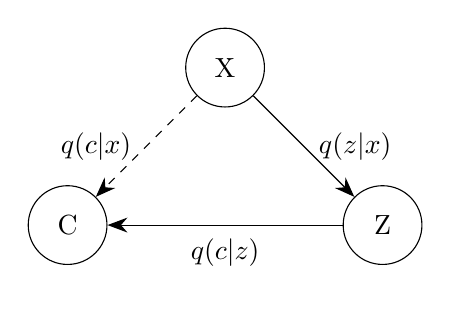
\begin{tikzpicture}[
    node distance=2cm,
    every node/.style={draw, circle, minimum size=1cm},
    >={Stealth[scale=1.5]}
]

% Nodes
\node (X) at (0,2) {X};
\node (Z) at (2,0) {Z};
\node (C) at (-2,0) {C};

% Edges with plain-text labels
\draw[->] (X) -- node[midway, right, draw=none, fill=none] {\( q(z|x) \)} (Z);
\draw[->] (Z) -- node[pos=0.5, yshift=-10pt, draw=none, fill=none] {\( q(c|z) \)} (C); % Slightly below
\draw[->, dashed] (X) -- node[midway, left, draw=none, fill=none] {\( q(c|x) \)} (C);

\end{tikzpicture}
    \caption{Directed Graphical Model}
    \label{fig:graphical_model}
\end{figure}


\begin{figure}[H]
    \centering
    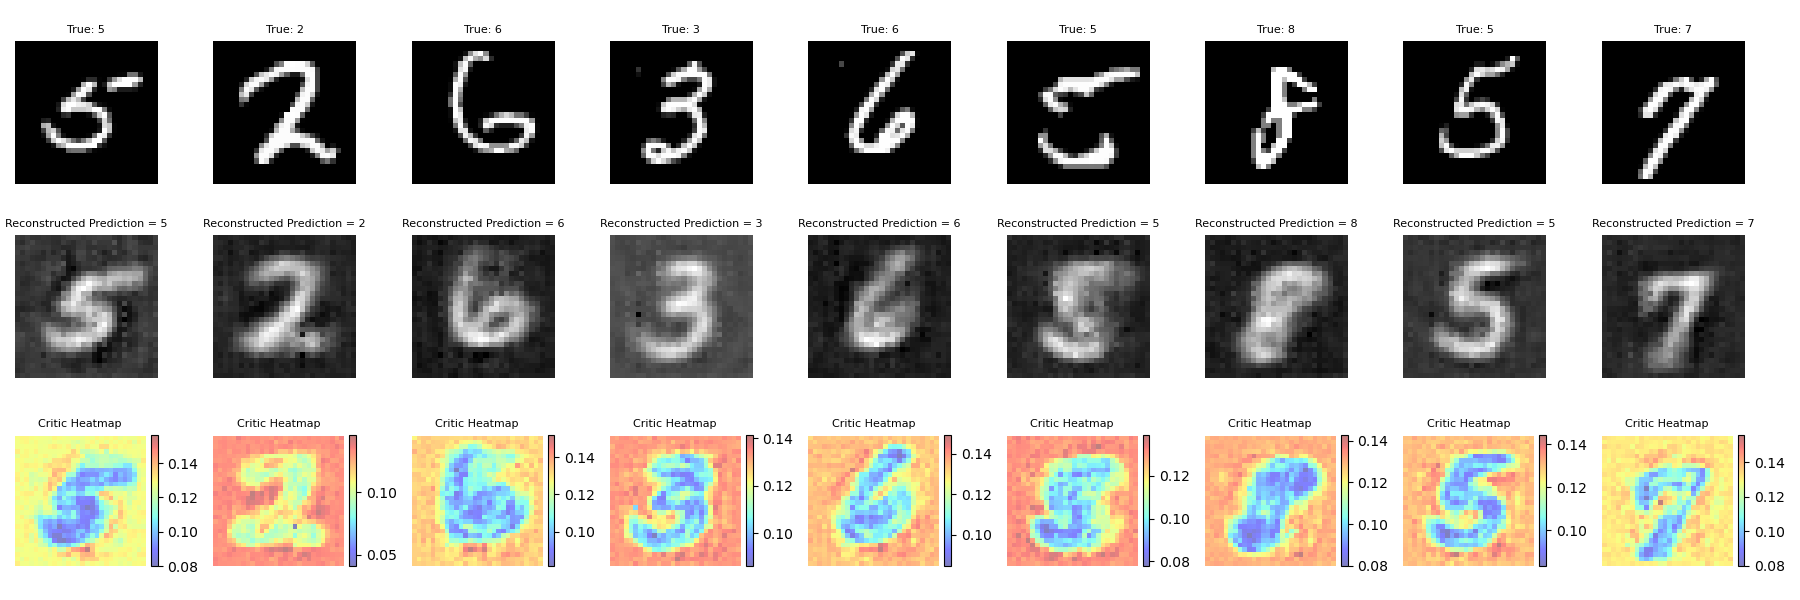
\includegraphics[width=\textwidth]{../fig/comparison_images_v1_cat_sum_training1.png}
    \caption{Example of VAE output, reconstruction, and critic heatmap in training set.}
    \label{fig:vae_example2}
\end{figure}

\begin{figure}[H]
    \centering
    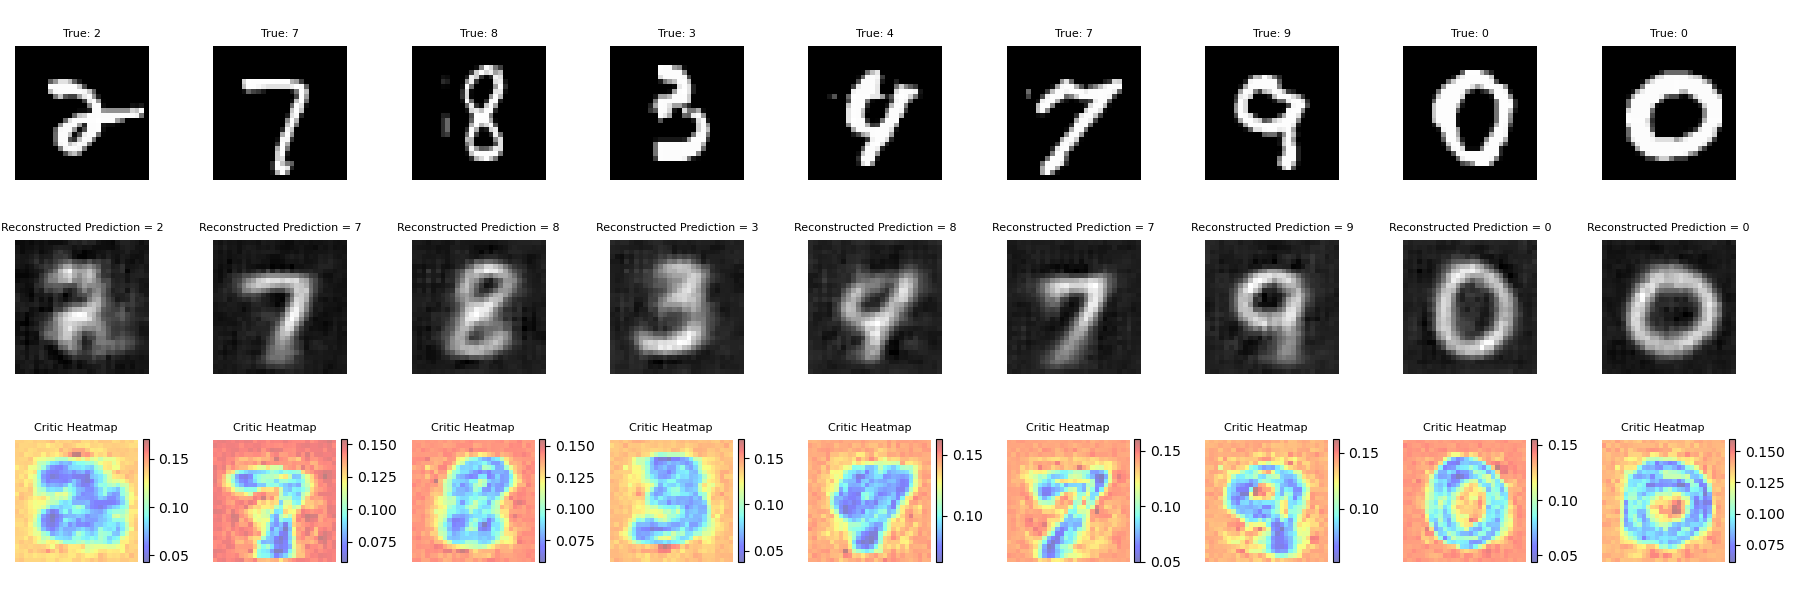
\includegraphics[width=\textwidth]{../fig/comparison_images_v1_cat_sum.png}
    \caption{Example of VAE output, reconstruction, and critic heatmap in testing set.}
    \label{fig:vae_example1}
\end{figure}


\section{Conclusion}
\ldots

123456

\newpage
\begin{footnotesize} %%Makes bib footnotesize text size
\singlespacing %%Makes single spaced
\bibliographystyle{ieeetr}
% \bibliographystyle{Phil_Review} %%bib style found in bst folder, in bibtex folder, in texmf folder.
\setlength{\bibsep}{5pt} %%Changes spacing between bib entries
\bibliography{Zotero} %%bib database found in bib folder, in bibtex folder
\thispagestyle{empty} %%Removes page numbers
\end{footnotesize} %%End makes bib small text size

\end{document}
